% Asset ID: FA21MaclaurinSeriesTikZ-001
% Topic ID: FA21MaclaurinSeries
% Unit: FA21 - Further A2 1 Pure Mathematics
% Topic code: FA21-FAF
% Related lesson file: FA21_maclaurin_series_lesson.md
% Related lesson section: Section 9.5 TikZ precise graph sketch
% Used placeholder:
% [VISUAL PLACEHOLDER: FA21MaclaurinSeriesTikZ-001 | Source: CCEA Maclaurin LO + DrFrost/Pearson graph idea | Insert from tikz/FA21MaclaurinSeriesTikZ-001.tex | Purpose: Provide a precise mathematical graph sketch of \(y=\sin x\), \(y=x\), \(y=x-\frac{x^3}{3!}\), and \(y=x-\frac{x^3}{3!}+\frac{x^5}{5!}\). The graph must include axes, origin label, and a highlighted neighbourhood around \(x=0\).]
%
% Source: CCEA Maclaurin LO boundary plus DrFrost/Pearson Maclaurin recap graph idea.
% Purpose: Precise graph sketch of y=sin x and successive Maclaurin approximations.
% Evidence status: Evidence-inspired and CCEA-syllabus-backed.

\documentclass[tikz,border=8pt]{standalone}
\usepackage{pgfplots}
\usepackage{amsmath}
\usepackage[T1]{fontenc}
\usepackage{lmodern}
\pgfplotsset{compat=1.18}

\definecolor{CanvasCream}{HTML}{FAF9F6}
\definecolor{PanelIvory}{HTML}{FFFFF0}
\definecolor{LineGrey}{HTML}{E5E5EA}
\definecolor{AccentGold}{HTML}{C5A059}
\definecolor{RichGold}{HTML}{D4AF37}
\definecolor{SoftRose}{HTML}{FBEFEF}
\definecolor{MathText}{HTML}{2C2C2E}
\definecolor{DeepOliveGold}{HTML}{8A7A47}

\begin{document}
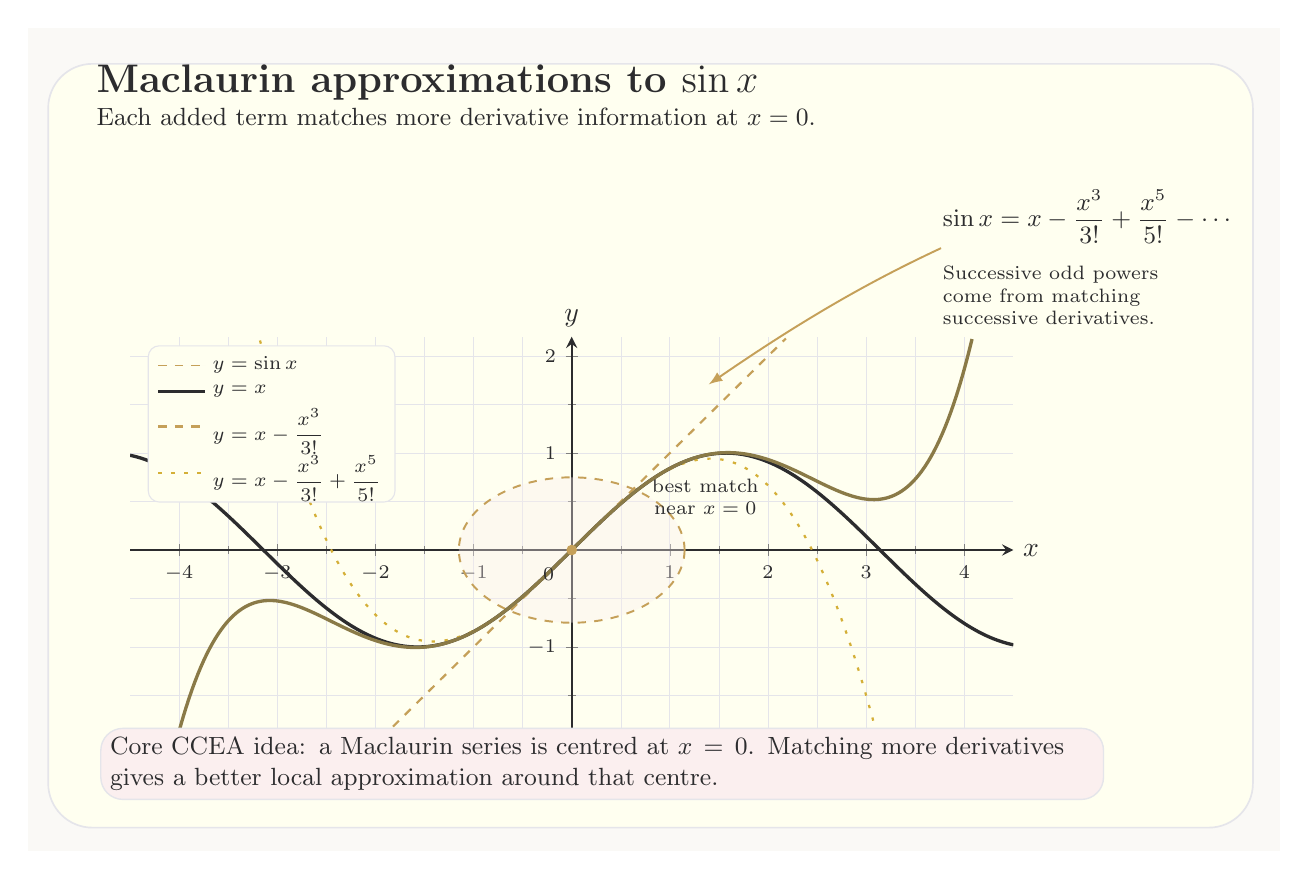
\begin{tikzpicture}
  \fill[CanvasCream] (-1.3,-1.1) rectangle (14.6,9.35);
  \node[fill=PanelIvory,draw=LineGrey,line width=0.6pt,rounded corners=16pt,minimum width=15.3cm,minimum height=9.7cm,anchor=south west] at (-1.05,-0.82) {};
  \node[anchor=west,text=MathText,font=\bfseries\Large] at (-0.55,8.65) {Maclaurin approximations to \(\sin x\)};
  \node[anchor=west,text=MathText,font=\small] at (-0.55,8.22) {Each added term matches more derivative information at \(x=0\).};

  \begin{axis}[
    width=12.8cm,height=7.0cm,at={(0,0.55)},xmin=-4.5,xmax=4.5,ymin=-2.2,ymax=2.2,
    axis lines=middle,axis line style={draw=MathText,line width=0.8pt},xlabel={\(x\)},ylabel={\(y\)},
    xlabel style={text=MathText,anchor=west},ylabel style={text=MathText,anchor=south},
    ticklabel style={font=\scriptsize,text=MathText},xtick={-4,-3,-2,-1,0,1,2,3,4},ytick={-2,-1,0,1,2},
    minor tick num=1,grid=both,major grid style={draw=LineGrey,line width=0.35pt},minor grid style={draw=LineGrey,line width=0.18pt},
    samples=300,domain=-4.5:4.5,restrict y to domain=-2.2:2.2,clip=true,
    legend style={draw=LineGrey,fill=PanelIvory,rounded corners=4pt,font=\scriptsize,text=MathText,at={(0.02,0.98)},anchor=north west},legend cell align=left]

    \addplot[draw=AccentGold,fill=SoftRose,fill opacity=0.35,line width=0.7pt,dashed,domain=0:360,samples=120] ({1.15*cos(x)},{0.75*sin(x)});
    \node[text=MathText,font=\scriptsize,align=center] at (axis cs:1.36,0.55) {best match\\near \(x=0\)};

    \addplot[MathText,very thick] {sin(deg(x))};
    \addlegendentry{\(y=\sin x\)}
    \addplot[AccentGold,thick,dashed] {x};
    \addlegendentry{\(y=x\)}
    \addplot[RichGold,thick,dash pattern=on 1.2pt off 3.5pt] {x - x^3/6};
    \addlegendentry{\(y=x-\dfrac{x^3}{3!}\)}
    \addplot[DeepOliveGold,very thick] {x - x^3/6 + x^5/120};
    \addlegendentry{\(y=x-\dfrac{x^3}{3!}+\dfrac{x^5}{5!}\)}
    \addplot[only marks,mark=*,mark size=1.7pt,color=AccentGold] coordinates {(0,0)};
    \node[anchor=north east,text=MathText,font=\scriptsize] at (axis cs:-0.08,-0.08) {\(0\)};
  \end{axis}

  \node[fill=SoftRose,draw=LineGrey,line width=0.5pt,rounded corners=8pt,text=MathText,font=\small,align=left,text width=12.5cm,anchor=west] at (-0.38,0.00)
  {Core CCEA idea: a Maclaurin series is centred at \(x=0\). Matching more derivatives gives a better local approximation around that centre.};

  \node[text=MathText,font=\small,align=left,anchor=west] at (10.2,6.95)
  {\(\displaystyle \sin x=x-\frac{x^3}{3!}+\frac{x^5}{5!}-\cdots\)};
  \draw[AccentGold,line width=0.7pt,-latex] (10.3,6.55) .. controls (9.55,6.20) and (8.70,5.75) .. (7.35,4.82);
  \node[text=MathText,font=\scriptsize,align=left,anchor=west] at (10.2,5.95) {Successive odd powers\\come from matching\\successive derivatives.};
\end{tikzpicture}
\end{document}
